
\chapter{Introduction}
\section{Motivation}

The upcoming High Luminosity phase of the Large Hadron Collider (LHC) \cite{LHC_machine_2008} offers unprecedented opportunities to explore new physics in both ATLAS \cite{collaboration_atlas_2008} and CMS \cite{CMS_2008}, with its increased luminosity enabling the collection of vast amounts of experimental data. Notably, from Run 2 to Run 3, the luminosity increased by approximately twofold \cite{Future_LHC}.

With a higher collision rate, the collider is expected to produce around 1 billion proton-proton (p-p) collisions per second, captured by detectors containing nearly 100 million readout channels. With only 25 nanoseconds between consecutive groups of colliding protons, new collisions occur even before the previous interactions have fully exited the detector. This massive volume of data not only represents a rich source for scientific discoveries but also poses immense challenges in terms of data processing, storage, and simulation requirements.

Simulation plays a critical role in high-energy physics, as it enables researchers to determine if experimental data aligns with theoretical models. Before delving into deeper analyses, every study must first validate that the observed data is consistent with both background expectations and the signal. This essential step ensures that we have a solid understanding of the main background and signal contributions to each channel, allowing us to apply suitable analysis strategies. However, the high computational demands of this simulation process create bottlenecks, especially as data rates increase. Thus, accelerating the simulation process without compromising accuracy is crucial for timely and reliable analysis.

\begin{figure}[H]
    \centering
    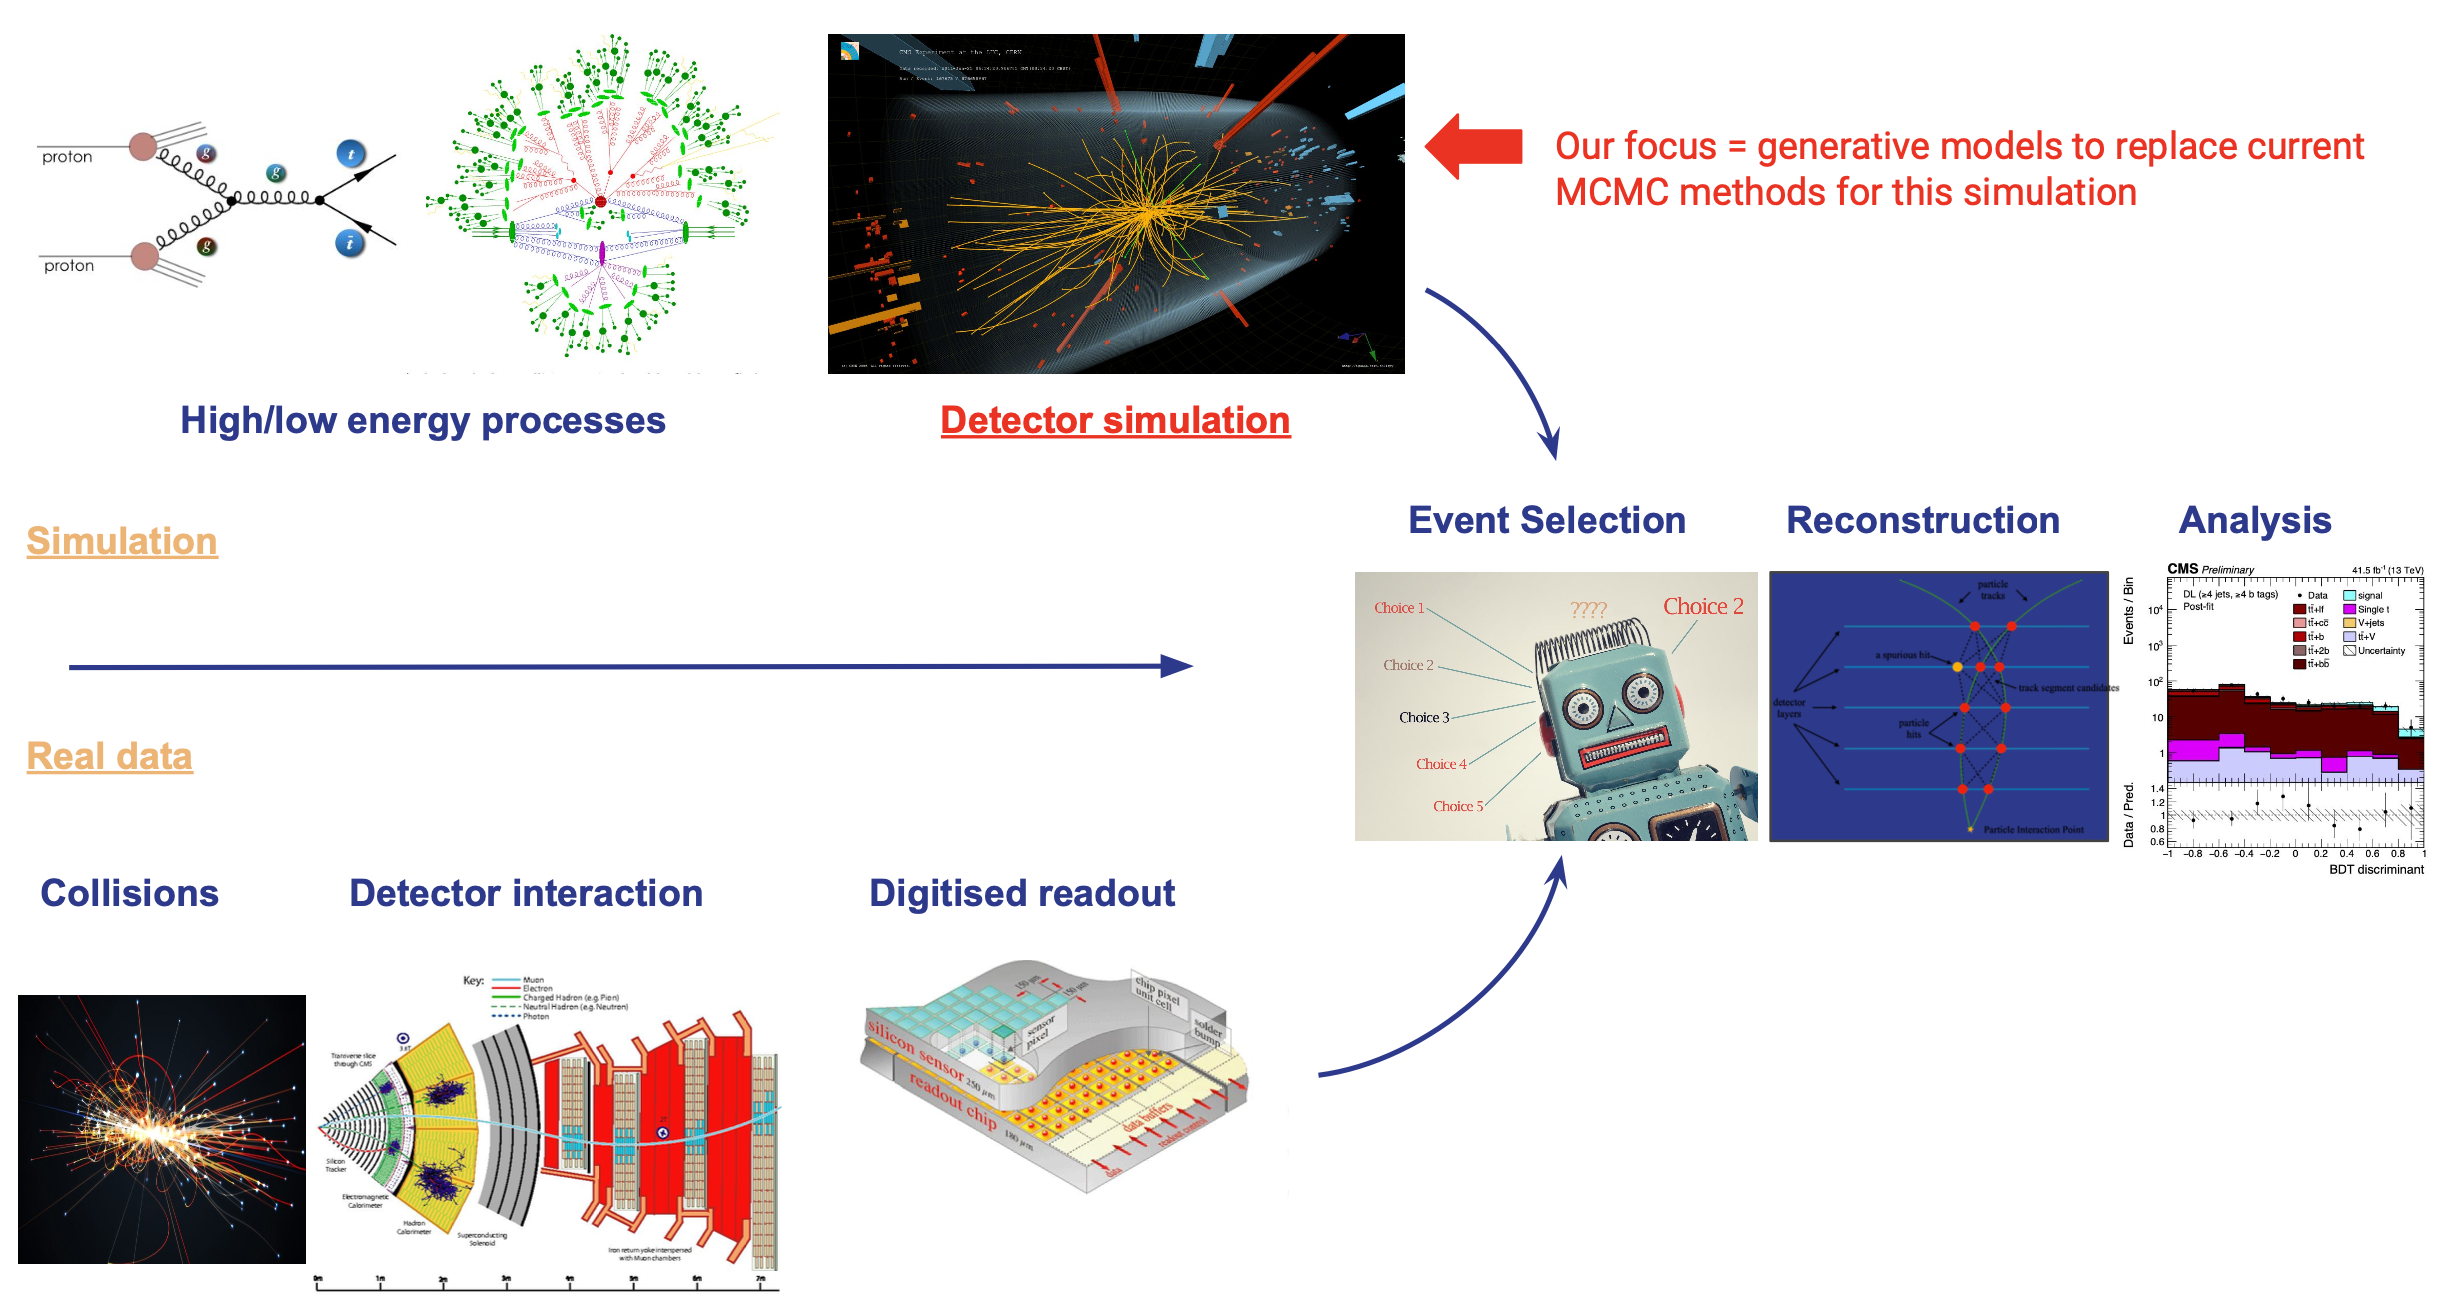
\includegraphics[width=0.7\textwidth]{Figures/simulation.png}
    \caption{The importance of simulation. credit: Joshuha Thomas-Wilsker}
    \label{fig:fig1}
\end{figure}

The simulation of particle interactions and detector responses, traditionally carried out by Monte Carlo methods and implemented with tools like Geant4 \cite{Geant4}, has been a foundational aspect of high-energy physics research. However, these methods are computationally intensive and struggle to keep pace with the data rates expected in the Run3 and even future. As the complexity of detector and collider setups continues to grow, so does the time required for full simulations, making it increasingly difficult to scale traditional techniques to meet the demands of modern experiments.

In response to the challenges posed by increasing data rates, generative models—especially diffusion models—have shown promising potential to accelerate simulations without sacrificing quality. Our goal is not to fully replace Geant4 simulations but rather to find a balance between accuracy and speed, as illustrated in Figure \ref{fast} . Recent works, including Yang et al.'s score-based models \cite{song2020} and other diffusion approaches in calorimeter simulations \cite{mikuni2021}, have achieved significant reductions in computation time while maintaining fidelity. Building on these innovations, our project introduces a novel model designed to generate 3D point clouds representing energy distributions across spatial coordinates in one step. Unlike previous models, which often focus on single-dimensional energy profiles (e.g., energy vs. z-coordinate), our approach captures the full 3D energy distribution in a single forward pass, allowing for rapid and comprehensive simulations that could match the data collection demands of high-luminosity experiments.

Detailed detector simulations are crucial in particle and nuclear physics data analysis. They allow researchers to compare particle-level predictions with observed data and to account for detector effects, making it possible to accurately interpret experimental results and compare them with theoretical predictions. Simulations also play a significant role in designing future experiments, guiding adjustments to optimize detector performance \cite{geant1, geant2}. Geant4-based simulations \cite{geant3} have become a standard tool in high-energy physics due to their precision, but achieving this precision is computationally demanding. Particle propagation in dense materials produces numerous secondary particles that undergo complex electromagnetic and nuclear interactions, making calorimeters—whose role is to measure deposited energy—the most challenging detectors to simulate accurately. In fact, a large portion of computing resources in high-energy physics is dedicated to simulating particle propagation in dense materials using Geant4.

The experiments at the Large Hadron Collider (LHC) generate billions of events per run, each with hundreds to thousands of individual calorimeter showers. Due to computing budget constraints, it is not feasible to use Geant4 simulations for all events, so experiments have developed fast simulation methods. These methods replace physics-based models with simpler parametric models calibrated to full simulations. While these fast simulations are efficient, their simplified parameterizations limit their accuracy, especially for modeling complex, high-dimensional correlations. Often, only a few one-dimensional observables are optimized, which may not fully capture the intricacies of particle interactions.

Deep learning provides a compelling alternative to traditional parametric models, with generative approaches like Generative Adversarial Networks (GANs) \cite{goodfellow2014}, Variational Autoencoders (VAEs) \cite{kingma2013}, and Normalizing Flows (NFs) \cite{dinh2016} increasingly adapted for fast detector simulations. GANs, for example, have demonstrated considerable speed and adaptability in generating calorimeter showers \cite{paganini2018} and are now even integrated into the ATLAS experiment’s fast simulation framework \cite{atlas2018}. Nonetheless, GANs present optimization challenges and can suffer from mode collapse,where the generator produces a narrow range of outputs, failing to capture the diversity of the data distribution. Conversely, NFs provide robust training and accurate density estimation, yet they remain computationally demanding when applied to high-dimensional data, which limits their practicality for simulating complex detector responses \cite{verheyen2021, verheyen2021b}.

In this work, we explore score-based generative models \cite{song2020}, which learn the gradient of the data density rather than the density itself, enabling a more flexible network architecture without requiring the Jacobian computation during training. This flexibility supports the use of bottleneck layers, reducing trainable parameters and improving scalability. Recent advances in score-based generative models have shown potential in calorimeter simulation, achieving a balance between high-dimensional fidelity and computational efficiency, making them suitable for ultra-fine calorimeters and other high-complexity datasets \cite{cms2017, cms2018}.

By leveraging score-based models, our project aims to address both the demands of the high-luminosity phase of the LHC and the limitations of traditional fast simulation methods. Our approach enhances accuracy by capturing full 3D spatial distributions while significantly reducing the time required for simulation, thus providing a scalable, reliable solution for next-generation collider experiments.

\begin{figure}[H]
    \centering
    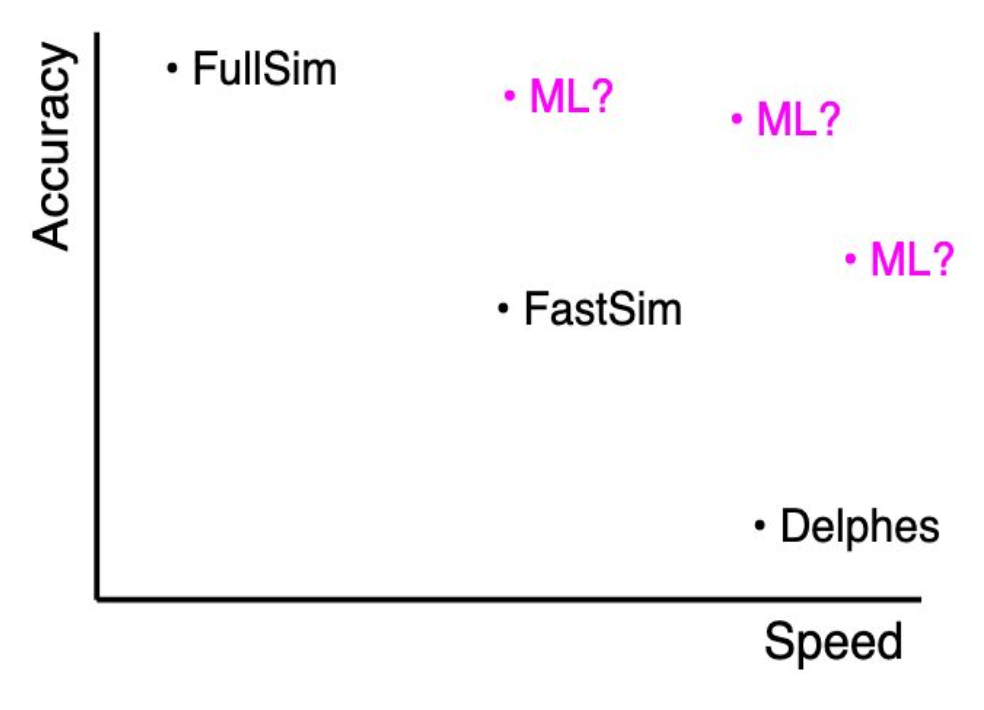
\includegraphics[width=0.7\textwidth]{Figures/fast.png}
    \caption{The balance between accuracy and speed in simulation. credit: Joshuha Thomas-Wilsker}
    \label{fast}
\end{figure}

\section{Challenges}

The generation of a 3D point cloud to depict energy deposition across spatial coordinates introduces unique challenges. Existing approaches primarily model the relationship between energy and a single spatial dimension, typically generating only partial representations of energy distributions. Our model, by contrast, aims to capture the complete three-dimensional energy profile in a single forward pass, which requires balancing high-dimensional fidelity and computational efficiency.

To achieve this goal, our model leverages advanced features, including Gaussian Fourier Projection for time encoding and mean-field attention mechanisms with a class token, in addition to conditional guidance based on incident energy. These architectural choices allow us to control both positional and energy distributions, addressing the intricacies of accurate 3D spatial modeling. However, managing the computational load and also let model learn every relation between each variables is quite hard.

This high-dimensional generative task requires careful conditioning to reflect realistic variations in energy deposition across multiple spatial coordinates, especially given the model’s need to dynamically adjust based on the incident energy. Achieving this balance involves a tradeoff between accuracy and computational load, as the high fidelity demanded in multi-dimensional output often requires extensive computation. Nevertheless, our optimized approach achieves up to a 100-fold speedup over traditional simulation methods, providing a scalable solution that addresses the needs of next-generation collider experiments.

In summary, our project seeks to address both the demands of high luminosity and the constraints of traditional simulations, aiming to bridge the gap between scalability and fidelity in particle shower simulations. Our advancements in 3D point cloud generation not only enhance the efficiency of simulations but also mark a step forward in producing realistic, high-dimensional data essential for future discoveries in high-energy physics.